
\noindent{\Large \bf Supplementary Material}

\bigskip

\section{Data collection}
1- Data collection: key words, clade (ordinal) metacharacters, Google Search terms, Google Search protocol, Google Search rarefaction curve.

\subsection{Public repositories}
We downloaded available matrices containing fossil and/or living mammal taxa from the three following data bases using the following list of keywords:

\texttt{Mammalia; Monotremata; Marsupialia; Placentalia; Macroscelidea; Afrosoricida; Tubulidentata; Hyracoidea; Proboscidea; Sirenia; Pilosa; Cingulata; Scandentia; Dermoptera; Primates; Lagomorpha; Rodentia; Erinaceomorpha; Soricomorpha; Cetacea; Artiodactyla; Cetartiodactyla; Chiroptera; Perissodactyla; Pholidota; Carnivora; Didelphimorphia; Paucituberculata; Microbiotheria; Dasyuromorphia; Peramelemorphia; Notoryctemorphia; Diprotodontia}.

Details about each public repository specific search option is listed below. Note that some matrices have been downloaded from more than one database but that it is not an issue since we are interested in the total number of living OTUs and that if some where present in more than one matrix, they still only counted as a unique OTU.

\subsubsection{Morphobank}
We accessed the Morphobank repository (\texttt{http://www.morphobank.org/}) on the 5th of December 2014 and used the keywords listed above in the search menue. We downloaded the data associated with each project matching with the keyword.

\subsubsection{Graeme Lloyd}
We accessed Graeme Lloyd's website repository (\texttt{http://graemetlloyd.com/}) on the 5th of December 2014 and downloaded all the matrices that were available with a direct download link in the mammal data section of the website (\texttt{http://graemetlloyd.com/matrmamm.html}).

\subsubsection{Ross Mounce}
We accessed Ross Mounce's GitHub repository (\texttt{https://github.com/rossmounce}) on the 2nd of December 2014 and downloaded every 601 matrix. We then ran a shell script to select only the matrices that had any text element that match with one of the search terms. To make the matrix selection more thorough, we ignored the keywords case as well as the latin suffix (\textit{ia}, \textit{ata}, \textit{ea}, and \textit{a}).

\subsection{Google scholars}
To make sure we didn't miss any extra matrix that wasn't available on one of these repository, we ran a Google Scholar search on the 5th of January. We used the following key words:

\texttt{\textit{order} ("morphology" OR "morphological" OR "cladistic") AND characters matrix paleontology phylogeny}

were \textit{order} was replaced by all the keywords listed above. For each 33 keywords, we selected the 20 first papers to match the Google search published since 2010 resulting in 660 papers. Among these papers, not all contained relevant data (discrete morphological characters AND mammalian data). We selected only the 20 first results per search term to avoid downloading articles that were to irrelevant. Among the 660 papers, only 50 contained a total of 425 extra living OTUs (figure ~\ref{Supp_figure_google_searches}).
Also we decided to select only the articles published since 2010 because nearly every one of the recent published matrix contains both a fraction of morphological characters and OTUs from previous studies. For example in primates the character \textit{p7} coded first by \cite{ross1998phylogenetic} is reused with the same living species in \cite{seiffert2003fossil}, \cite{marivaux2005anthropoid}, \cite{seiffert2005basal}, \cite{bloch2007new}, \cite{bloch2007new}, \cite{kay2008anatomy}, \cite{silcox2008biogeographic}, \cite{seiffert2009convergent}, \cite{tabuce2009anthropoid}, \cite{boyer2010astragalar}, \cite{seiffert2010fossil}, \cite{marivaux2013djebelemur} and \cite{ni2013oldest}.

\begin{figure}[!htbp]
\centering
    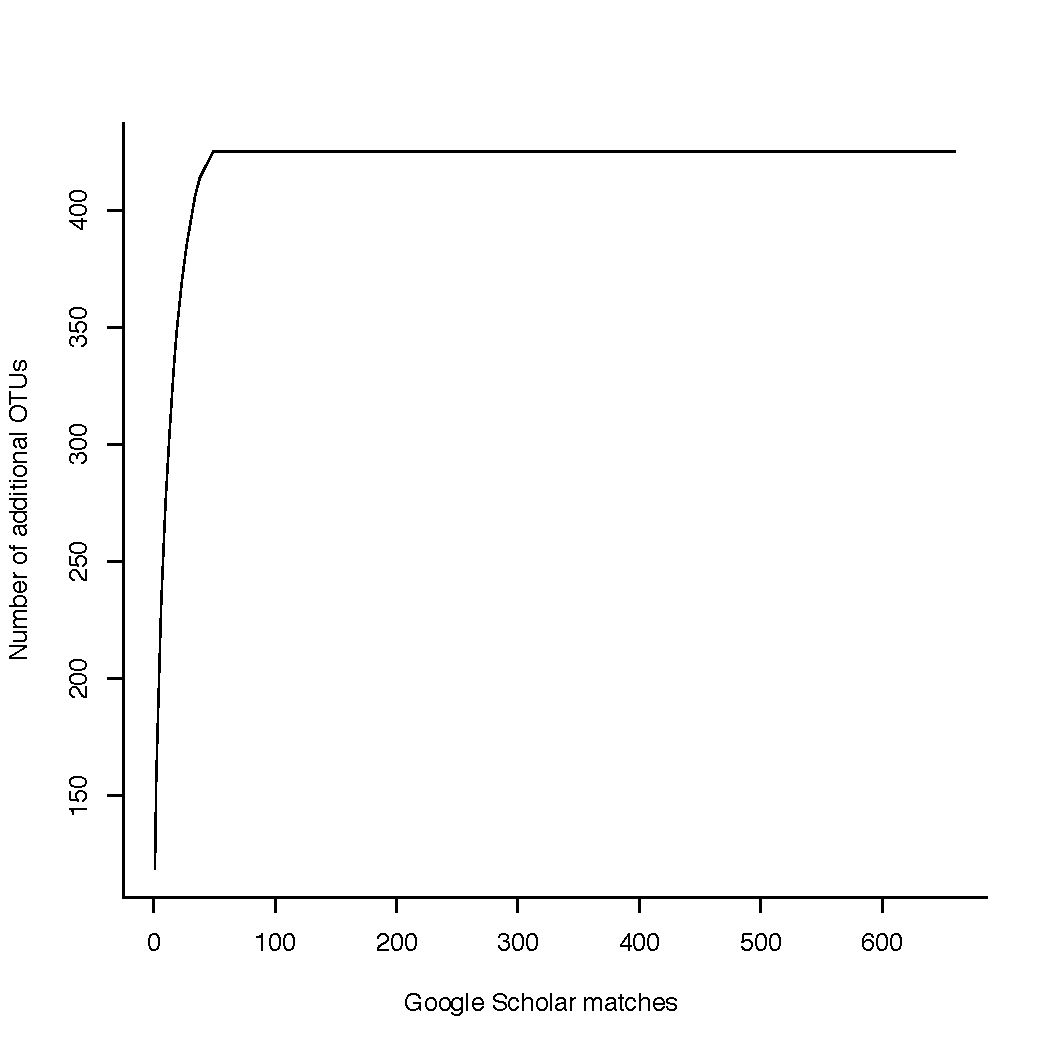
\includegraphics[width=1\textwidth]{Supplementary/Supp_figure_google_searches.pdf}
\caption{Google searches additional OTUs rarefaction curve. The x axis represent the number of google scholar matches (papers, books or abstracts) and the y axis represents the cumulative number of additional living OTUs per google scholar match.}
\label{Supp_figure_google_searches}
\end{figure}

\subsection{Standardising the matrices}
We transformed all the non-nexus matrices (tnt, word, excel, jpeg) to nexus format manually. We then cleaned the nexus matrices by removing any extra information (trees, continuous characters, morphological characters description, molecular data) to end up with nexus matrices containing only the discrete morphological data. We then manually fixed the wrong bionomial names format (e.g. \textit{H. sapiens}) into the correct ones (e.g. \textit{Homo sapiens}) using the abbreviation list in the concerned publications. 

\subsection{Selecting the living OTUs}
Finally we applied a taxonomic matching algorithm to classify the OTUs as either living or fossil. The algorithm is matching every OTU name from every matrix with one of the following taxonomic references: the list of taxa from the Fritz \textit{et al.} supertree (2009) \cite{FritzTree}; the taxonomic list from the Wilson and Reeder's Mammals Species of the World (2005) \cite{wilson2005mammal} and the list of all the mammal fossil from the Paleobio Database (\texttt{http://paleobiodb.org/cgi-bin/bridge.pl?a=login}) accessed on the 13th of Janurary 2015. The OTUs that matched with one of the two first references were considered as living OTUs, the OTUs matching with the third reference were considered as fossil OTUs, finally, the OTUs matching with non of the references were discarded (figure ~\ref{Supp_figure_Taxonomic_algorithm}).

\begin{figure}[!htbp]
\centering
    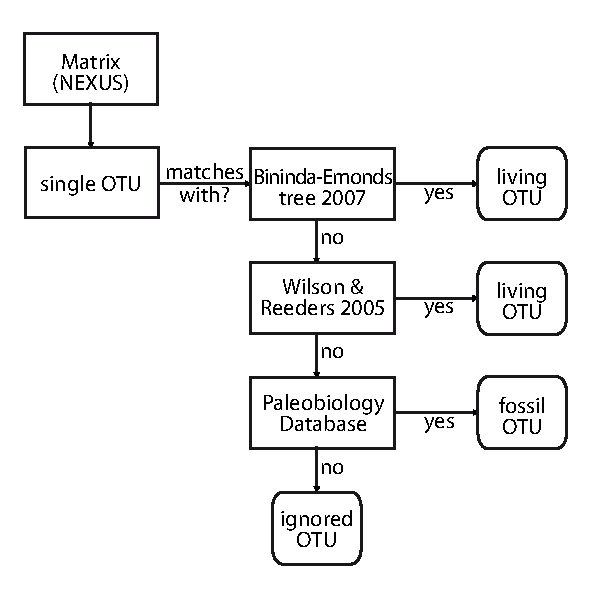
\includegraphics[width=1\textwidth]{Supplementary/Supp_figure_Taxonomic_algorithm.pdf}
\caption{Taxonomic matching algorithm used in this study. For each matrix, each operational taxonomic units (OTU) is matched with the super tree from Fritz 2009. If the OTU matches, then it is classified as living. Else it is matched with the Wilson \& Reeders 2005 taxonomy list. If the OTU matches, then it is classified as living. Else it is matched with the Paleo Database list of mammals. If the OTU matches, then it is classified as fossil. Else it is ignored.}
\label{Supp_figure_Taxonomic_algorithm}
\end{figure}

\bibliographystyle{vancouver}
\bibliography{Supp_References}


\section{Data structure}
%Tables
%Figures

\section{Supplementary results}
